\documentclass{article}
\usepackage[margin=25mm]{geometry} % 25 mm margins all around
\usepackage{graphicx} % for pdf figures


\begin{document}
%
%
\section*{Fig. S1}
\begin{figure}[ht]
	\centering
	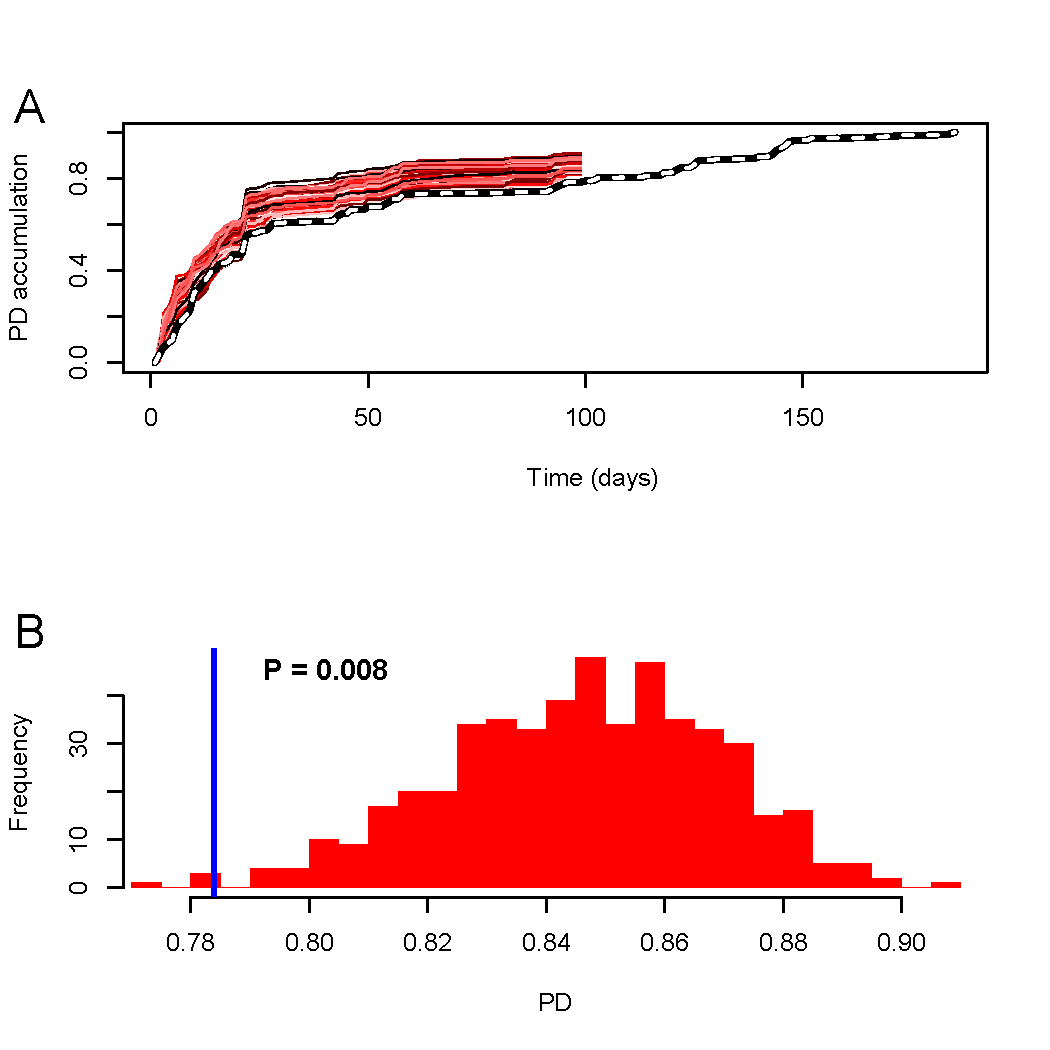
\includegraphics[scale=0.80]{../Fig_S1.pdf}
\end{figure}
Significance testing for the female feces data set. Plot A shows the empirical phylodiversity accumulation (dashed; same as Fig. 1A) but with neutral model surrogate data sets shown in different shades of red. These are produced by running the neutral model 500 times, to generate a distribution of phylodiversity values under \(D = 0\) (Plot B). As with all surrogate data sets, these are run until time \(m\) (see Parameter Estimation section of Materials and Methods). Empirical phylodiversity at time \(m\) (blue line) is compared to the distribution of neutral model phylodiversities at time \(m\) (red histogram), and a \(P\)-value is calculated as the proportion of neutral phylodiversities more extreme than the empirical value. 
\newpage
%
%
\section*{Fig. S2}
\begin{figure}[ht]
	\centering
	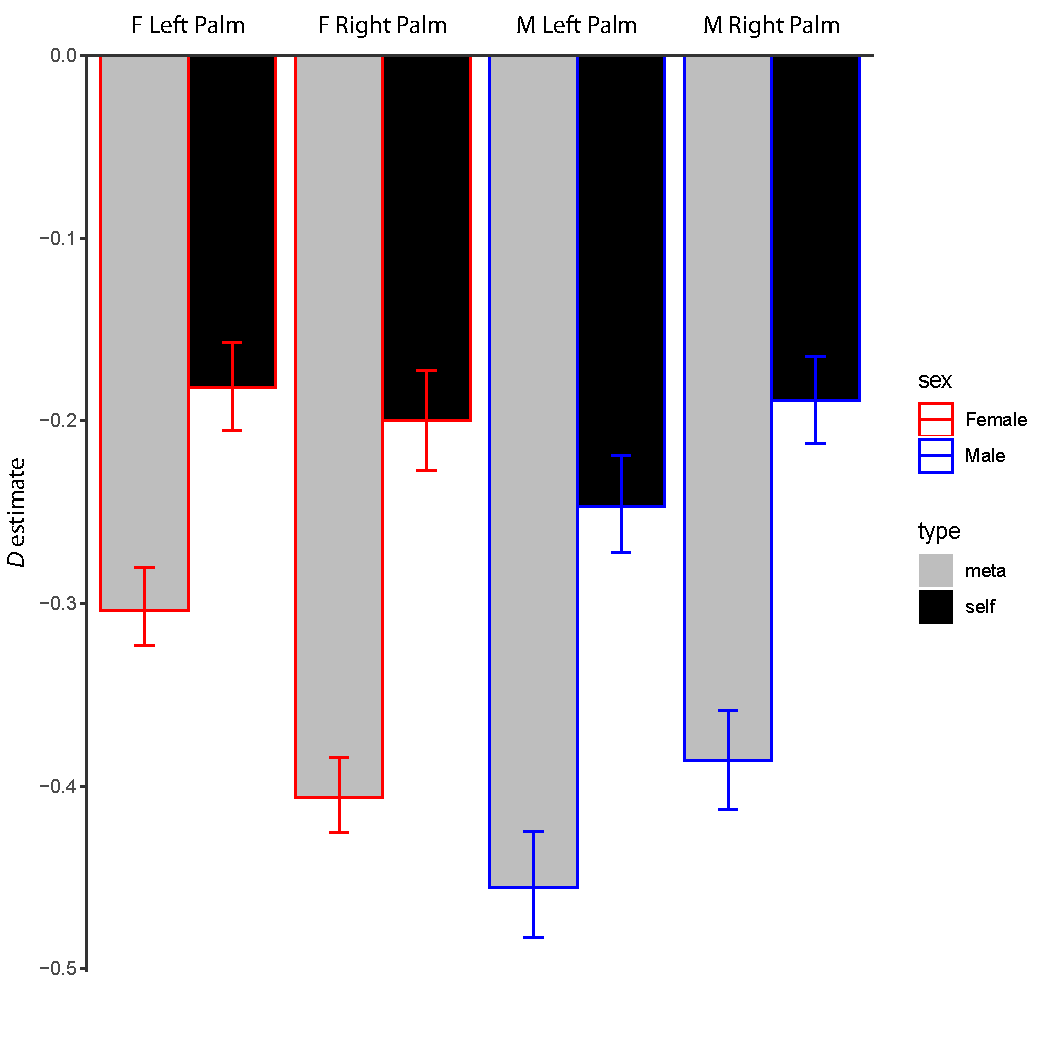
\includegraphics[scale=0.80]{../Fig_S2.pdf}
\end{figure}
Comparison of "self" vs "meta" model results from palm communities. "Self" (black) models were run identically to Fig. 2, but "meta" (gray) models were run where the species pool for each palm community surrogate data set was composed of all zOTUs observed across all four palm data sets. The difference between the "self" \(D\) estimate (generated above) and the "meta" \(D\) estimate (estimated with a metapopulation of zOTUs) is related to the exclusivity of recruitment into the community. In other words, if we were to estimate similar \(D\) values for both the "meta" and "self" analyses, the inclusion of extra species in the species pool would be of little importance to the model, and we would learn that it would make little difference to community assembly patterns if the species pool really was composed of the "meta" set.
\newpage
%
%
\section*{Fig. S3}
\begin{figure}[ht]
	\centering
	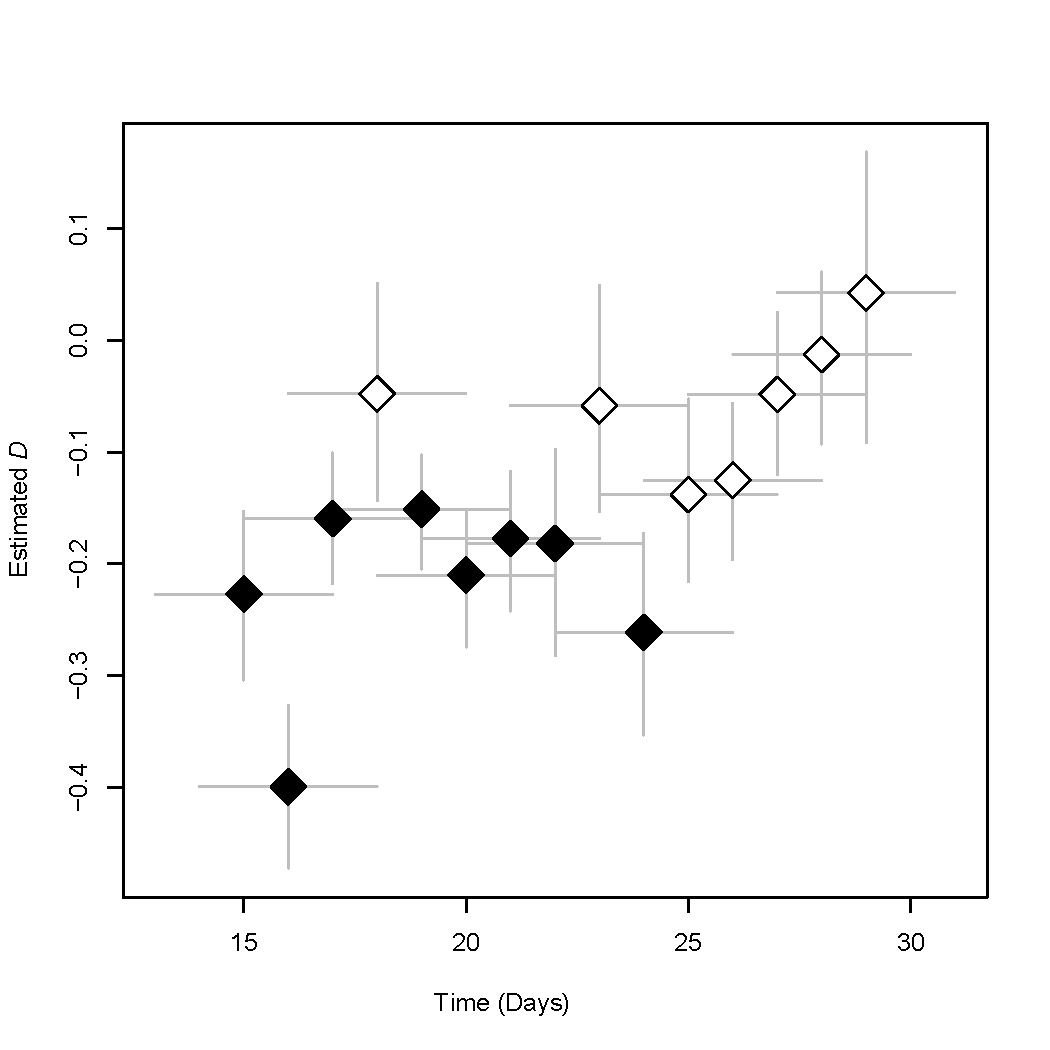
\includegraphics[scale=0.80]{../Fig_S3.pdf}
\end{figure}
Sliding window analysis of male right palm data over 19 consecutive samples. We ran our model on each window of 5 continuous days (15 windows), in order to see how \(D\) varied over time. We only conducted this analysis for the section of samples that were sampled every day, so that comparisons between windows would not be confounded by window size. This analysis was done to demonstrate a potential use case for our model, and not to test any specific hypothesis. Filled shapes represent windows that were significantly different than the neutral model. Vertical bars represent 95\% confidence intervals for \(D\) estimate, and horizontal bars represent window size.
\newpage
%
%
\section{Fig. S4}
\begin{figure}[ht]
	\centering
	\includegraphics[scale=0.80]{../Fig_S4.pdf}
\end{figure}
\(D\) estimates of Finnish infant datasets. All but two subjects exhibited significant phylogenetic underdispersion. The two subjects that were not significantly different from the neutral model were both in the antibiotics cohort, which is comprised of infants that were treated with frequent antibiotics, almost all for ear infections. There was no significant difference between \(D\) values for the two groups. 
\newpage
%
%
\section*{Fig. S5}
\begin{figure}[ht]
	\centering
	\includegraphics[scale=0.80]{../Fig_S5.pdf}
\end{figure}
Relationship of \(D\) estimate to total zOTU richness, total phylodiversity, number of timepoints sampled, and initial phylodiversity (of first sample) for Finnish infant data. No statistically significant correlation was detected in any of these four analyses. 
%
\end{document}